\documentclass[../main.tex]{subfiles}
\begin{document}
\subsection{Introduzione}
Una funzione $f$ è una legge che associa ad ogni elemento $x$ di un insieme di partenza $A$ un \textbf{unico} elemento $y$ di un insieme di arrivo $B$.
\begin{center}
    \begin{tikzpicture}
        %sets A and B
        \draw (0,0) ellipse (1 and 2);
        \draw (5,0) ellipse (1 and 2);
        \node at (0, 2.3) {$A$};
        \node at (5,2.3) {$B$};
        \node at (2.5,0.3) {$f$};
        
        %set A
        \node at (0,0) {$\bullet$};
        \node at (-0.2,0.2) {$x$};

        
        %set B
        \node at (5,0) {$\bullet$};
        \node at (5.2,0.2) {$y$};
        
        %arrows
        \draw[->] (0.2,0) -- (4.8,0);
    \end{tikzpicture}
    \begin{align*}
        f:A& \longrightarrow B \\
        x& \longmapsto y = f(x)
    \end{align*}
\end{center}
$x$ è detto elemento di $A$ associato a $y$, elemento di $B$. \\

\subsubsection{Esempi}
\begin{enumerate}
    \item \begin{align*}
        f: \mathbb{R}& \longrightarrow \mathbb{R} \\
        x& \longmapsto y=3x-2 \\
        x&=5 \Rightarrow y=3\cdot5-2=13 \\
        &\Rightarrow f \text{ è una funzione}
    \end{align*}
    \item \begin{align*}
        f: \mathbb{R}& \longrightarrow \mathbb{R} \\
        x& \longmapsto y=\sqrt{x} \\
        x&=4 \Rightarrow y=\sqrt{4}=2 \\
        x&=-4 \Rightarrow y=\sqrt{-4} \\
        &\sqrt{-4} \text{ non esiste in } \mathbb{R} \\
        &\Rightarrow f \text{ non è una funzione}
    \end{align*}
    \item \begin{align*}
        f: \mathbb{R}& \longrightarrow \mathbb{R} \\
        x& \longmapsto y=\pm x^2 \\
        x&=3 \Rightarrow y=\pm 3^2=\pm 9 \\
        x&=+9 \\
        x&=-9 \\
    \end{align*}
    L'argomento possiede due immagini, $f$ \textbf{non} è una funzione
\end{enumerate}

\pagebreak
\subsection{Dominio}
Sia $f$ una funzione. Il suo dominio $D(f)$ è l'insieme di tutti gli elementi $x$ per i quali $f(x)$ è ben definita.

\subsubsection{Esempi}
\begin{enumerate}
    \item \begin{align*}
        f:D(&f) \rightarrow \mathbb{R} \\
        &x \mapsto f(x)=1/x \\
        D(&f)= \mathbb{R} \backslash \{0\}
    \end{align*}
    \item \begin{align*}
        f:D(&f) \rightarrow \mathbb{R} \\
        &x \mapsto y=\sqrt{x+2} \Rightarrow D(f)=\lbrack -2;+ \infty \lbrack
    \end{align*}
    \item \begin{align*}
        f:D(&f) \rightarrow \mathbb{R} \\
        &x \mapsto \frac{1}{\sqrt{x+2}} \Rightarrow D(f)= \rbrack -2;+\infty \lbrack
    \end{align*}
    \item \begin{align*}
        f:D(&f) \rightarrow \mathbb{R} \\
        &x \mapsto y=3x-1 \Rightarrow D(f)= \mathbb{R}
    \end{align*}
\end{enumerate}

\textbf{Nota:} il dominio è l'insieme di partenza più grande possibile, per trovarlo occorre innanzitutto analizzare le limitazioni della funzione, escludere i valori non validi e riportare l'insieme più grande possibile che non comprenda quei valori.
\begin{center}
    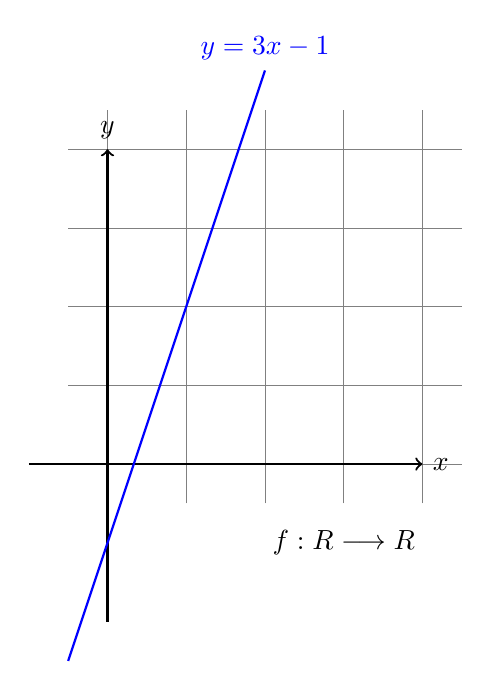
\begin{tikzpicture}
        % Disegna la griglia
        \draw[very thin, gray] (-0.5,-0.5) grid (4.5,4.5);
        
        % Disegna assi
        \draw[thick,->] (-1,0) -- (4,0) node[right] {$x$}; % Asse x
        \draw[thick,->] (0,-2) -- (0,4) node[above] {$y$}; % Asse y

        % Disegna la funzione y = 3x - 2
        \draw[domain=-0.5:2,smooth,variable=\x,blue,thick] 
        plot ({\x},{3*\x-1}) node[above] {$y = 3x - 1$};

        \node at (3, -1) {$f:\mathbb{R}\longrightarrow \mathbb{R}$};
    \end{tikzpicture} \hspace{2cm}
    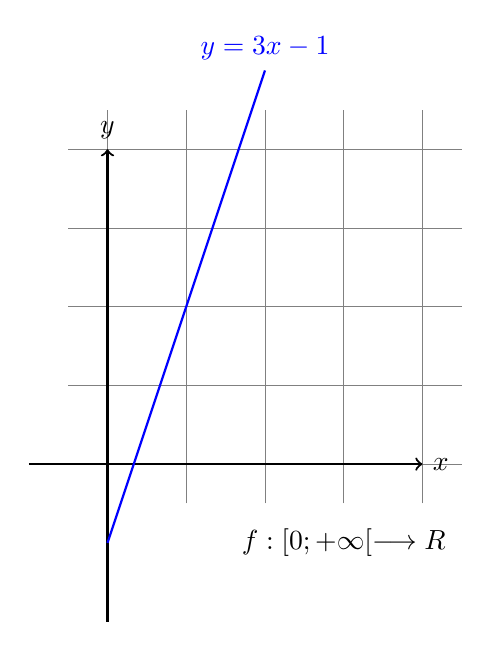
\begin{tikzpicture}
        % Disegna la griglia
        \draw[very thin, gray] (-0.5,-0.5) grid (4.5,4.5);
        
        % Disegna assi
        \draw[thick,->] (-1,0) -- (4,0) node[right] {$x$}; % Asse x
        \draw[thick,->] (0,-2) -- (0,4) node[above] {$y$}; % Asse y

        % Disegna la funzione y = 3x - 2
        \draw[domain=0:2,smooth,variable=\x,blue,thick] 
        plot ({\x},{3*\x-1}) node[above] {$y = 3x - 1$};

        \node at (3, -1) {$f:\lbrack 0; +\infty \lbrack \longrightarrow \mathbb{R}$};
    \end{tikzpicture}
\end{center}

\pagebreak
\subsection{Insieme immagini}
Sia $f:A \rightarrow B$ una funzione. Il suo insieme delle immagini è definito come segue:
$$
    Im(f)= \{ y=f(x)|x \in A \}
$$
Generalmente $x$ indica gli argomenti e $y$ le immagini, nello schema visto nell'introduzione $B$
rappresenta l'insieme delle immagini. Tutti gli elementi di $A$ sono associati ad un elemento di $B$,
ma non per forza viceversa.

\subsubsection{Esempi}
\begin{align*}
    f: \mathbb{R}& \longrightarrow \mathbb{R} \\
    x& \longmapsto y=3x-1 \\
    &\Rightarrow Im(f)=\mathbb{R}
\end{align*}
In questo caso per trovare $Im$ guardiamo il grafico.

\begin{center}
    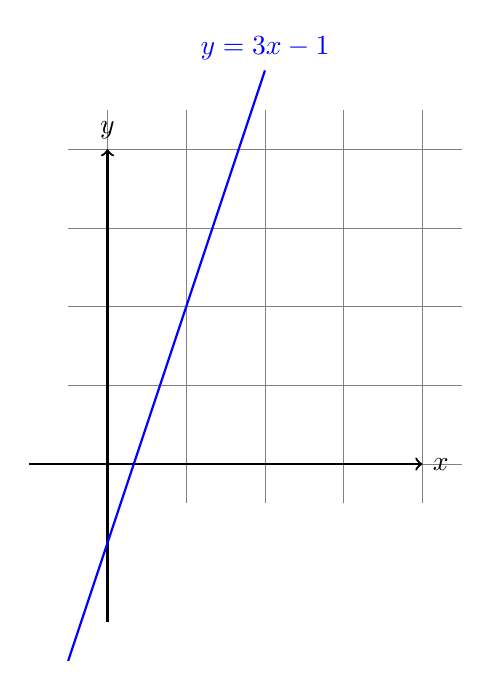
\begin{tikzpicture}
        % Disegna la griglia
        \draw[very thin, gray] (-0.5,-0.5) grid (4.5,4.5);
        
        % Disegna assi
        \draw[thick,->] (-1,0) -- (4,0) node[right] {$x$}; % Asse x
        \draw[thick,->] (0,-2) -- (0,4) node[above] {$y$}; % Asse y

        % Disegna la funzione y = 3x - 2
        \draw[domain=-0.5:2,smooth,variable=\x,blue,thick] 
        plot ({\x},{3*\x-1}) node[above] {$y = 3x - 1$};
    \end{tikzpicture}
\end{center}

\begin{align*}
    g: \mathbb{R}& \longrightarrow \mathbb{R} \\
    x& \longmapsto x^2-2 \\
    &\Rightarrow Im(g)= \lbrack -2; + \infty \lbrack \\
    &= \lbrack y_v;+ \infty \lbrack
\end{align*}
In questo caso trattandosi di una \textbf{parabola}, per determinare $Im(g)$ guardiamo il vertice.

\textbf{Nota:} Non esiste una ricetta o una procedura precisa per trovare l'$Im$ di una funzione, non è come per il dominio.

\pagebreak
\subsection{Grafico di una funzione}
Sia $f:A \rightarrow B$ una funzione. Il suo grafico $G(f)$ è l'insieme dei punti 
$$
    G(f)= \{ (a;f(a)) | a \in A \}
$$

\begin{figure}[h]
    \centering
    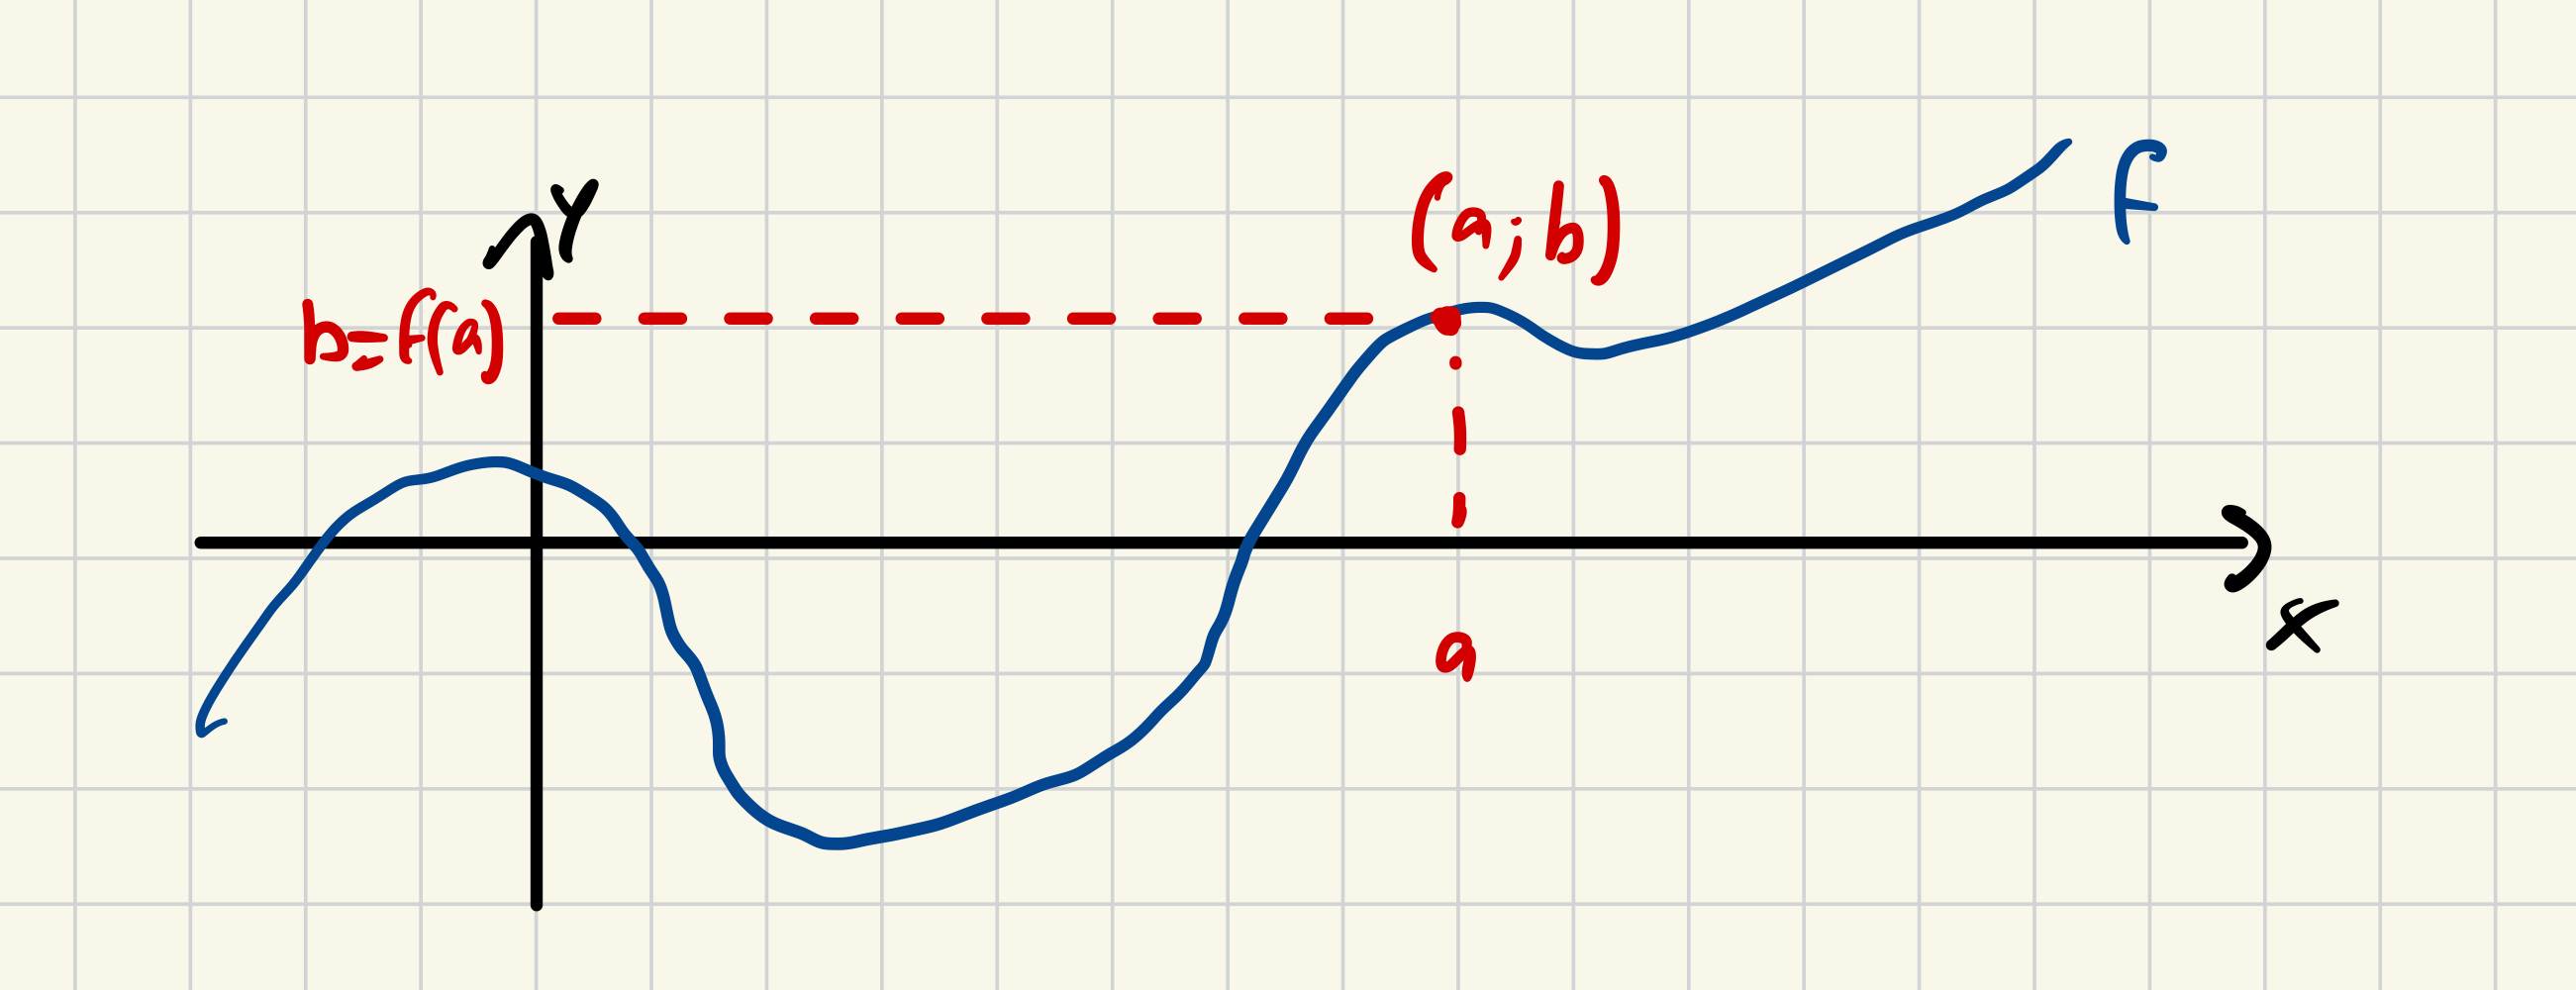
\includegraphics[width=0.8\textwidth]{../images/graficoFunzione.jpeg}
\end{figure}
$(a;b) \in G(f) \Leftrightarrow b = f(a)$, Un punto appartiene al grafico se e solo se $b=f(a)$

\textbf{Nota:} possiamo verificare se una funzione esiste dal suo grafico controllando che per ogni $x$ ci sia \textbf{soltanto} una $y$.
\vspace{1cm}


\subsection{Operazioni con le funzioni}
\subsubsection{Somma - Sottrazione}
Esempio:
\begin{align*}
    f(x)&=\sqrt{x+1} \Rightarrow D(f)=\lbrack-1;+\infty\lbrack \\
    g(x)&=\frac{1}{x}\Rightarrow D(g)=\mathbb{R} \backslash \{0\} \\
    (f\pm g)(x)&=\sqrt{x+1}\pm \frac{1}{x} \\
    \Rightarrow D(f+g)&=\lbrack-1;+\infty\lbrack \backslash \{0\} \\
    &=D(f)\cap D(g)
\end{align*}

In generale
\begin{align*}
    (f\pm g)(x) = f(x)\pm g(x)\\
    D(f\pm g) = D(f) \cap D(g) 
\end{align*}

\subsubsection{Prodotto}
\begin{align*}
    (f \cdot g)(x) = f(x) \cdot g(x) \\
    D(f \cdot g) = D(f) \cap D(g)  
\end{align*}

\subsubsection{Divisione}
La divisione non è solo l'intersezione tra le due funzioni.

\pagebreak
\subsection{Composizione di funzioni}
SCHEMA

\begin{align*}
    f: B \longrightarrow C \\
    g: A \longrightarrow B \\
\end{align*}
La funzione
\begin{align*}
    f \circ  g: A \longrightarrow& C \\
    x \longrightarrow& (f \circ  g)(x) = f(g(x))
\end{align*}
è detta \textbf{composizione di f con g} ($f$ composto $g$).

\textbf{Nota:} In generale $f \circ g \neq g \circ  f $, la composizione di funzioni non è commutativa. 

\subsection{Funzione inversa}

\end{document}